\documentclass[14pt]{extbook}
\usepackage{multicol, enumerate, enumitem, hyperref, color, soul, setspace, parskip, fancyhdr} %General Packages
\usepackage{amssymb, amsthm, amsmath, latexsym, units, mathtools} %Math Packages
\everymath{\displaystyle} %All math in Display Style
% Packages with additional options
\usepackage[headsep=0.5cm,headheight=12pt, left=1 in,right= 1 in,top= 1 in,bottom= 1 in]{geometry}
\usepackage[usenames,dvipsnames]{xcolor}
\usepackage{dashrule}  % Package to use the command below to create lines between items
\newcommand{\litem}[1]{\item#1\hspace*{-1cm}\rule{\textwidth}{0.4pt}}
\pagestyle{fancy}
\lhead{Progress Quiz 7}
\chead{}
\rhead{Version C}
\lfoot{3510-5252}
\cfoot{}
\rfoot{Summer C 2021}
\begin{document}

\begin{enumerate}
\litem{
First, find the equation of the line containing the two points below. Then, write the equation in the form $ y=mx+b $ and choose the intervals that contain $m$ and $b$.\[ (-9, 6) \text{ and } (-8, 10) \]\begin{enumerate}[label=\Alph*.]
\item \( m \in [3, 9] \hspace*{3mm} b \in [14, 16] \)
\item \( m \in [3, 9] \hspace*{3mm} b \in [-42, -40] \)
\item \( m \in [-9, 3] \hspace*{3mm} b \in [-24, -18] \)
\item \( m \in [3, 9] \hspace*{3mm} b \in [39, 43] \)
\item \( m \in [3, 9] \hspace*{3mm} b \in [16, 22] \)

\end{enumerate} }
\litem{
Write the equation of the line in the graph below in Standard Form $Ax+By=C$. Then, choose the intervals that contain $A, B, \text{ and } C$.
\begin{center}
    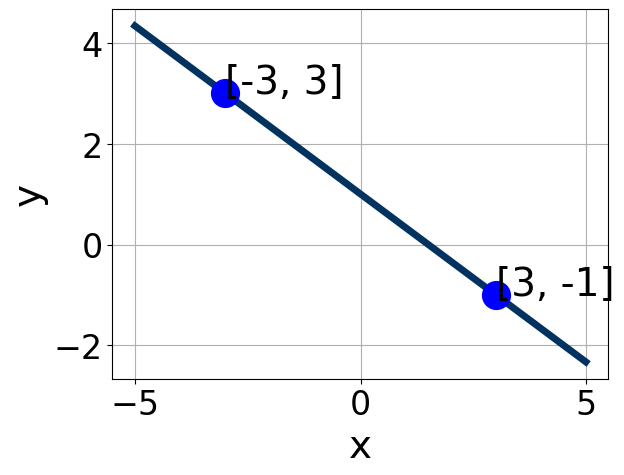
\includegraphics[width=0.5\textwidth]{../Figures/linearGraphToStandardCopyC.png}
\end{center}
\begin{enumerate}[label=\Alph*.]
\item \( A \in [0.9, 2.82], \hspace{3mm} B \in [2.1, 3.2], \text{ and } \hspace{3mm} C \in [2.9, 4.18] \)
\item \( A \in [-0.75, 0.8], \hspace{3mm} B \in [-0.9, 2.3], \text{ and } \hspace{3mm} C \in [0.89, 1.33] \)
\item \( A \in [-0.75, 0.8], \hspace{3mm} B \in [-1.2, 0.9], \text{ and } \hspace{3mm} C \in [-1.63, -0.12] \)
\item \( A \in [0.9, 2.82], \hspace{3mm} B \in [-4.5, -2.4], \text{ and } \hspace{3mm} C \in [-3.28, -2.97] \)
\item \( A \in [-3.19, -0.91], \hspace{3mm} B \in [-4.5, -2.4], \text{ and } \hspace{3mm} C \in [-3.28, -2.97] \)

\end{enumerate} }
\litem{
Solve the equation below. Then, choose the interval that contains the solution.\[ -12(7x -2) = -6(-14x + 16) \]\begin{enumerate}[label=\Alph*.]
\item \( x \in [-0.59, -0.33] \)
\item \( x \in [0.38, 0.58] \)
\item \( x \in [0.67, 0.89] \)
\item \( x \in [-0.24, 0] \)
\item \( \text{There are no real solutions.} \)

\end{enumerate} }
\litem{
First, find the equation of the line containing the two points below. Then, write the equation in the form $ y=mx+b $ and choose the intervals that contain $m$ and $b$.\[ (-9, -5) \text{ and } (-10, -7) \]\begin{enumerate}[label=\Alph*.]
\item \( m \in [1.7, 4.1] \hspace*{3mm} b \in [11.7, 15.01] \)
\item \( m \in [1.7, 4.1] \hspace*{3mm} b \in [3.34, 5.29] \)
\item \( m \in [1.7, 4.1] \hspace*{3mm} b \in [-13.21, -12.4] \)
\item \( m \in [-3, -1.1] \hspace*{3mm} b \in [-28.17, -26.87] \)
\item \( m \in [1.7, 4.1] \hspace*{3mm} b \in [1.52, 3.14] \)

\end{enumerate} }
\litem{
Write the equation of the line in the graph below in Standard Form $Ax+By=C$. Then, choose the intervals that contain $A, B, \text{ and } C$.
\begin{center}
    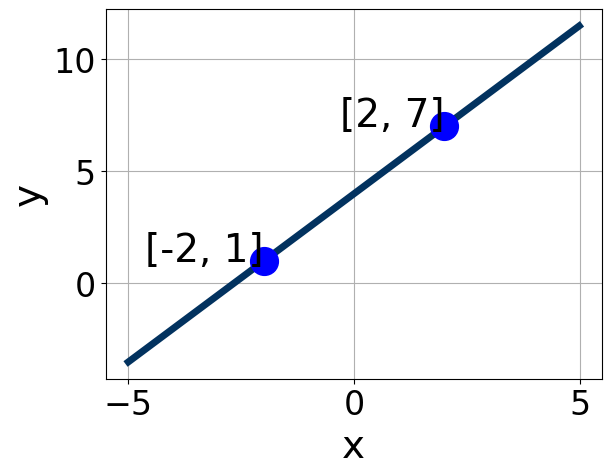
\includegraphics[width=0.5\textwidth]{../Figures/linearGraphToStandardC.png}
\end{center}
\begin{enumerate}[label=\Alph*.]
\item \( A \in [-2.07, -1.15], \hspace{3mm} B \in [-1.44, -0.95], \text{ and } \hspace{3mm} C \in [-5.5, -3.4] \)
\item \( A \in [-3.29, -2.8], \hspace{3mm} B \in [1.96, 2.69], \text{ and } \hspace{3mm} C \in [7.3, 10.1] \)
\item \( A \in [1.55, 3.68], \hspace{3mm} B \in [1.96, 2.69], \text{ and } \hspace{3mm} C \in [7.3, 10.1] \)
\item \( A \in [1.55, 3.68], \hspace{3mm} B \in [-2.26, -1.9], \text{ and } \hspace{3mm} C \in [-8.9, -7.4] \)
\item \( A \in [-2.07, -1.15], \hspace{3mm} B \in [0.54, 1.34], \text{ and } \hspace{3mm} C \in [3.4, 5.6] \)

\end{enumerate} }
\litem{
Solve the equation below. Then, choose the interval that contains the solution.\[ -15(8x + 3) = -9(14x -6) \]\begin{enumerate}[label=\Alph*.]
\item \( x \in [-2.8, -0.5] \)
\item \( x \in [-1.2, 0.1] \)
\item \( x \in [0.5, 2.6] \)
\item \( x \in [15.7, 17.6] \)
\item \( \text{There are no real solutions.} \)

\end{enumerate} }
\litem{
Solve the linear equation below. Then, choose the interval that contains the solution.\[ \frac{-4x + 7}{8} - \frac{7x + 3}{5} = \frac{-6x -3}{4} \]\begin{enumerate}[label=\Alph*.]
\item \( x \in [16.5, 19.5] \)
\item \( x \in [0.2, 2.2] \)
\item \( x \in [5.56, 8.56] \)
\item \( x \in [1.56, 4.56] \)
\item \( \text{There are no real solutions.} \)

\end{enumerate} }
\litem{
Find the equation of the line described below. Write the linear equation in the form $ y=mx+b $ and choose the intervals that contain $m$ and $b$.\[ \text{Parallel to } 5 x - 8 y = 12 \text{ and passing through the point } (-4, -3). \]\begin{enumerate}[label=\Alph*.]
\item \( m \in [0.74, 3.04] \hspace*{3mm} b \in [-1.67, 0.09] \)
\item \( m \in [-0.16, 0.63] \hspace*{3mm} b \in [0.59, 1.56] \)
\item \( m \in [-2.11, -0.52] \hspace*{3mm} b \in [-5.65, -5.1] \)
\item \( m \in [-0.16, 0.63] \hspace*{3mm} b \in [-0.06, 0.58] \)
\item \( m \in [-0.16, 0.63] \hspace*{3mm} b \in [-1.67, 0.09] \)

\end{enumerate} }
\litem{
Solve the linear equation below. Then, choose the interval that contains the solution.\[ \frac{6x -7}{7} - \frac{-3x + 9}{5} = \frac{3x -3}{8} \]\begin{enumerate}[label=\Alph*.]
\item \( x \in [11.3, 13.9] \)
\item \( x \in [-0.4, 2] \)
\item \( x \in [2, 2.9] \)
\item \( x \in [-1.2, -0.9] \)
\item \( \text{There are no real solutions.} \)

\end{enumerate} }
\litem{
Find the equation of the line described below. Write the linear equation in the form $ y=mx+b $ and choose the intervals that contain $m$ and $b$.\[ \text{Perpendicular to } 7 x - 4 y = 8 \text{ and passing through the point } (-3, 2). \]\begin{enumerate}[label=\Alph*.]
\item \( m \in [-0.5, 0.9] \hspace*{3mm} b \in [3.52, 4.84] \)
\item \( m \in [-1.11, 0.04] \hspace*{3mm} b \in [4.56, 5.52] \)
\item \( m \in [-2.96, -0.9] \hspace*{3mm} b \in [0.2, 0.5] \)
\item \( m \in [-1.11, 0.04] \hspace*{3mm} b \in [-0.97, 0.16] \)
\item \( m \in [-1.11, 0.04] \hspace*{3mm} b \in [0.2, 0.5] \)

\end{enumerate} }
\end{enumerate}

\end{document}